\documentclass[12pt]{article}

\usepackage[utf8x]{inputenc}
\usepackage[english]{babel}

\usepackage{amssymb,amsmath,amsthm,amsfonts}
\usepackage{calc}
\usepackage{float}
\usepackage{graphicx}
\usepackage{subfigure}
\usepackage{gensymb}
\usepackage{url}
\usepackage[utf8x]{inputenc}
\usepackage[T1]{fontenc}
\usepackage{amsmath}
\usepackage{graphicx}
\graphicspath{{images/}}
\usepackage{parskip}
\usepackage{fancyhdr}
\usepackage{vmargin}
\usepackage{etoolbox}
\usepackage{flafter}
\patchcmd{\thebibliography}{\section*}{\section}{}{}
\setmarginsrb{3 cm}{2.5 cm}{3 cm}{2.5 cm}{1 cm}{1.5 cm}{1 cm}{1.5 cm}

\title{Prospector Sea Floor Mapping System}					
\author{UM}										


\makeatletter
\let\thetitle\@title
\let\theauthor\@author
\let\thedate\@date
\makeatother

\pagestyle{fancy}
\fancyhf{}
\rhead{\theauthor}
\lhead{\thetitle}
\cfoot{\thepage}

\begin{document}

%%%%%%%%%%%%%%%%%%%%%%%%%%%%%%%%%%%%%%%%%%%%%%%%%%%%%%%%%%%%%%%%%%%%%%%%%%%%%%%%%%%%%%%%%

\begin{titlepage}
	\centering
    \vspace*{0.0 cm}
    \textsc{\LARGE User Manual}\\[2.0 cm]
	\textsc{\Large Software Engineering and Project}\\[0.5 cm]			
	\textsc{\large University of Adelaide}\\[0.5 cm]
	\rule{\linewidth}{0.2 mm} \\[0.4 cm]
	{ \huge \bfseries \thetitle}\\
	\rule{\linewidth}{0.2 mm} \\[1.5 cm]
	
	\begin{minipage}{0.4\textwidth}
		\begin{center} \large
			Navdeep Singh (1660360)\linebreak
			Liang Yuan (1679380)\linebreak
			Zeqi Fu (1680895)\linebreak
			Tao Zhang (1680974)\linebreak
			Lili Wu (1683229)\linebreak
			Yi Lin (1682781)\linebreak
            Yann Frizenschaf (1162562)\linebreak
			\end{center}
	\end{minipage}\\[2 cm]
	
	{\large Semester 2, 2016}\\[2 cm]
 
	\vfill
	
\end{titlepage}

\pagenumbering{roman}

\begin{table}
\begin{tabular}{ | p{0.12\textwidth}| p{0.24\textwidth}| p{0.15\textwidth}| p{0.25\textwidth}|p{0.10\textwidth}|}
\hline
\multicolumn{5}{|c|}{\textbf{Revision History}}\\
\hline
\textbf \textbf{Date} &  \textbf\textbf{Name} &  \textbf\textbf{Student ID} & \textbf\textbf {Updates} & \textbf\textbf{Version} \\
\hline
19th Oct 2016 & Navdeep Singh & 1660360 & Added the basic structure of draft  & 0.1\\
\hline
20th Oct 2016 & Liang Yuan & 1679380 & add detail manual  & 0.2\\
\hline
26th Oct 2016 & Navdeep Singh & 1660360 & Added Screenshots and Details & 0.3\\
\hline
29th Oct 2016 & Yann Frizenschaf & 1162562 & Edits for release & 1.0\\
\hline
\end{tabular}

\end{table}


\clearpage 

\pagebreak
\tableofcontents
\pagebreak

\pagenumbering{arabic}
\section{Abstract}
This document is the User Manual for the Prospector Sea Floor Mapping System (SFM). It is designed to introduce a novice user to the user of the SFM Operations Graphical User Interface (GUI) to the various functions of the system including control of the robot prototype and map file import/export.

\section{Introduction}
\subsection{Overview}
 
The Prospector SFM system enables Map exploration through remote, autonomous control of a robotic vehicle which facilitates data acquisition. The primary goals of the software platform are therefore:
\begin{itemize}
\item to enable a human operator to send appropriate commands to the robot via a graphical user interface (GUI) in order to initiate autonomous exploration of the survey area (and intervene when necessary); and 
\item extract the gathered data via the same GUI into a XML file format.
\end{itemize}

\subsection{Purpose}

The purpose of this document is to detail the User Manual for the Prospector Seafloor Mapping System (SFM), developed for SeaFaults. It contains the details of how to connect to robot, how to perform a mapping operation and how to use the GUI.
\subsection{Scope}

This document defines the User manual  for the software component
of the SFM system only.

\subsection{Assumptions}

\begin{itemize}{}
\item The Machine running the GUI will have the Java 8 runtime environment pre-installed.
\item The operator will know the current IP address of the robot.
\item The robot will be powered on and connected to an appropriate Bluetooth or Wifi network.

\end{itemize}

\section{Human Interface Design}\label{GUI}

\subsection{Overview of the User Interface}
An overview of the GUI is shown in Figure \ref{fig:GUI}. The GUI consists of four main panels (clockwise from far left of the figure):
\begin{itemize}
\item The map panel, including the map legend, which shows the current state of the mapping operation
\item The control panel, consisting of arrow buttons for robot control, mode selection drop-down menu, destination entry fields, map loading and saving buttons, and robot manual position correction fields.
\item The information panel, which displays system state information
\item The connection panel, used to connect to the robot.
\end{itemize}
\subsection{Detailed Design of the User Interface}
\begin{figure}[H]
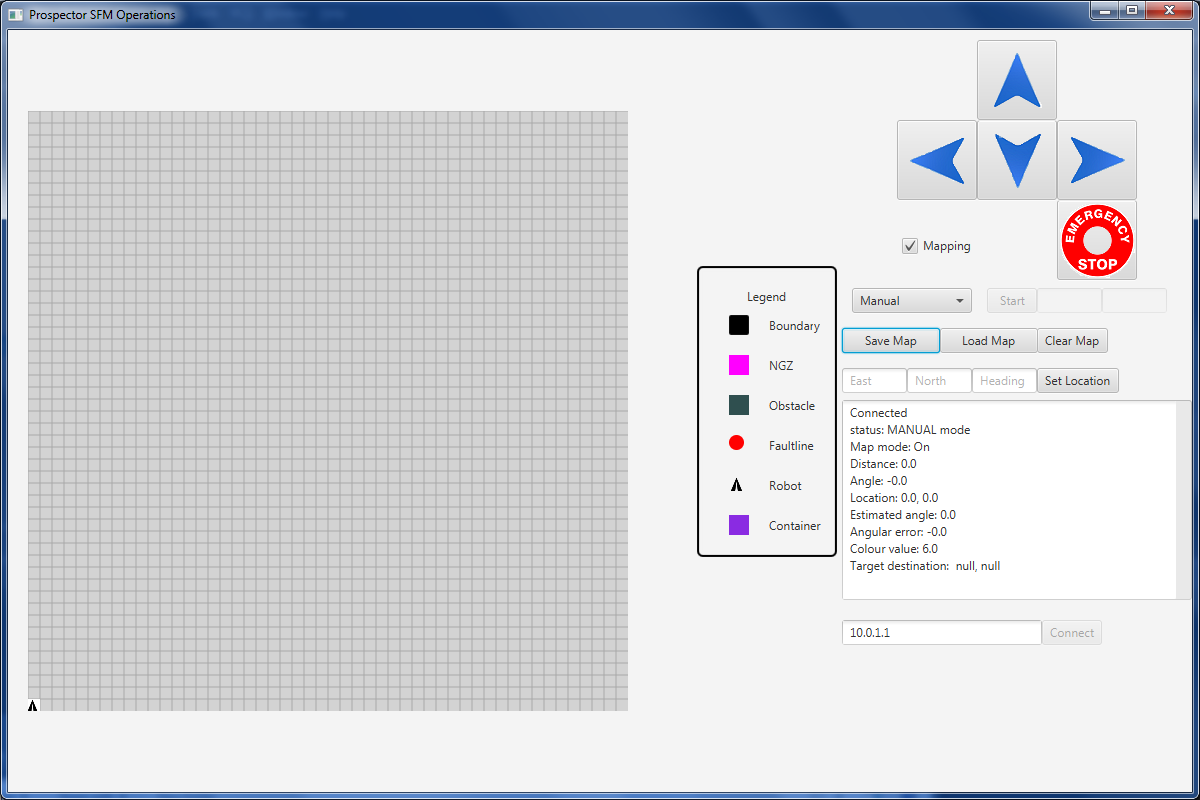
\includegraphics[width=\textwidth]{connected_ready.png}
\caption{User interface}
  \label{fig:GUI}
\end{figure}
\subsubsection{Connection field}
The user interface provides an input for user to input the IP address of the robot, in order to connect to robot, show below:
\begin{figure}[H]
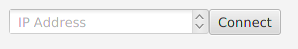
\includegraphics[width=\textwidth]{connect.png}
\caption{Connect}
  \label{fig:Connect}
\end{figure}

\subsubsection{Control mode}
The user interface provides the function that user can choose the control mode, including automatic mode, manual mode and move-to-point mode. When user chooses the automatic mode, the four direction buttons are dim, and the emergency button is light, shows as figure \ref{fig:Automatic_mode}. When user chooses manual mode, all control buttons are light, shows as figure \ref{fig:Manual_mode} . When user chooses move-to-point mode, the four direction buttons are dim, the emergency button is light. In addition, user need to input the point, shows as figure \ref{fig:Move_to_point_mode}.

\begin{figure}[H]
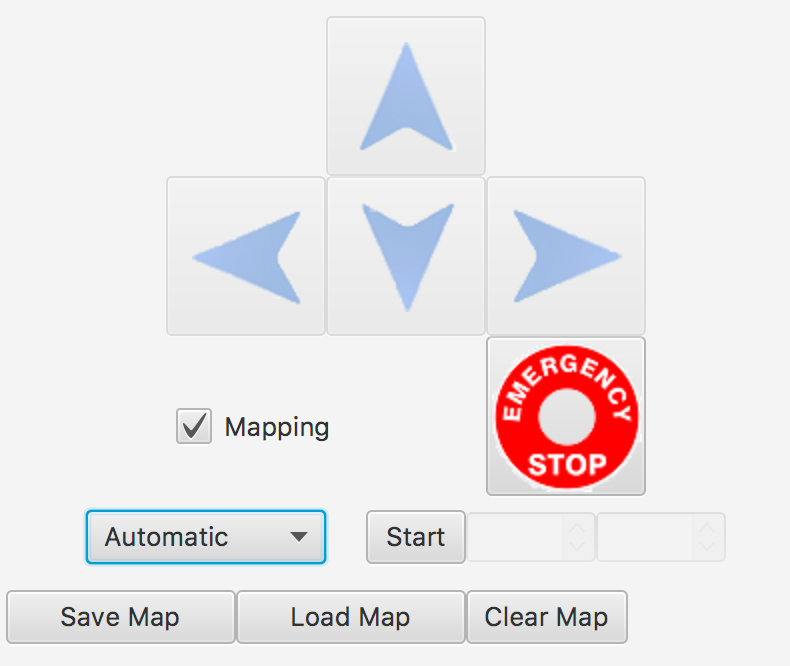
\includegraphics[width=\textwidth]{Automatic_mode.png}
\caption{Automatic Mode}
  \label{fig:Automatic_mode}
\end{figure}
\begin{figure}[H]
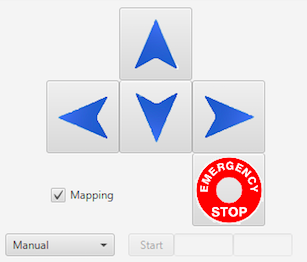
\includegraphics[width=\textwidth]{Manual_mode.png}
\caption{Manual Mode}
  \label{fig:Manual_mode}
\end{figure}
\begin{figure}[H]
\includegraphics[width=\textwidth]{move_to_point.png}
\caption{Move to Point}
  \label{fig:Move_to_point_mode}
\end{figure}

\subsubsection{Map operation}
The user interface provides three buttons in terms of map operation. The "Save Map" button is to save the map that has been drawn by robot, the "Load Map" button is to load the map that has provided, and the "Clear Map" button is to the current map, show below:
\begin{figure}[H]
\centering
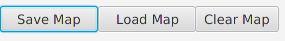
\includegraphics[width=\textwidth]{map.png}
\caption{Save Map 1 }
  \label{fig:Save_map1}
  \end{figure}
  \begin{figure}[H]
  \centering
  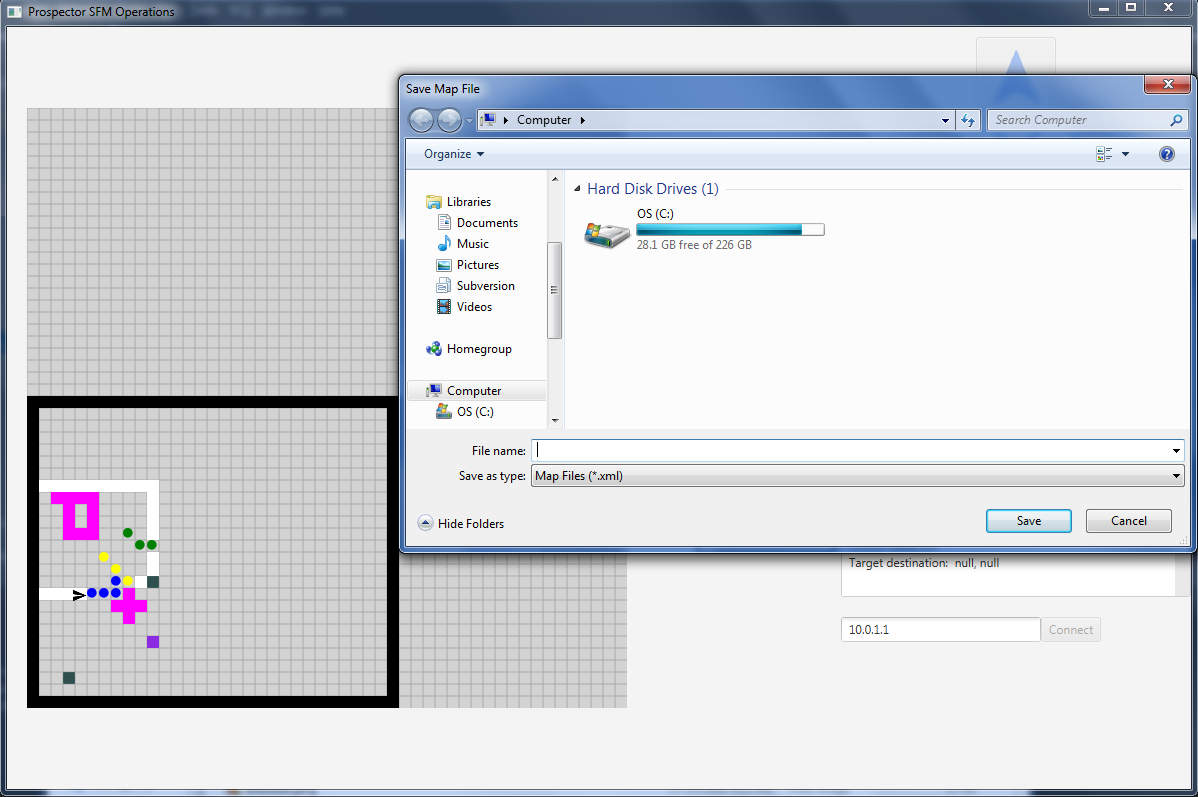
\includegraphics[width=\textwidth]{save_map.png}
  \caption{Save Map 2}
  \label{fig:Save_map2}
\end{figure}

\clearpage



\subsubsection{Location setting}
The user interface provide an input field for user to set the start location. Users need to type the location, and put the robot at that point, show below:
\begin{figure}[H]
\centering
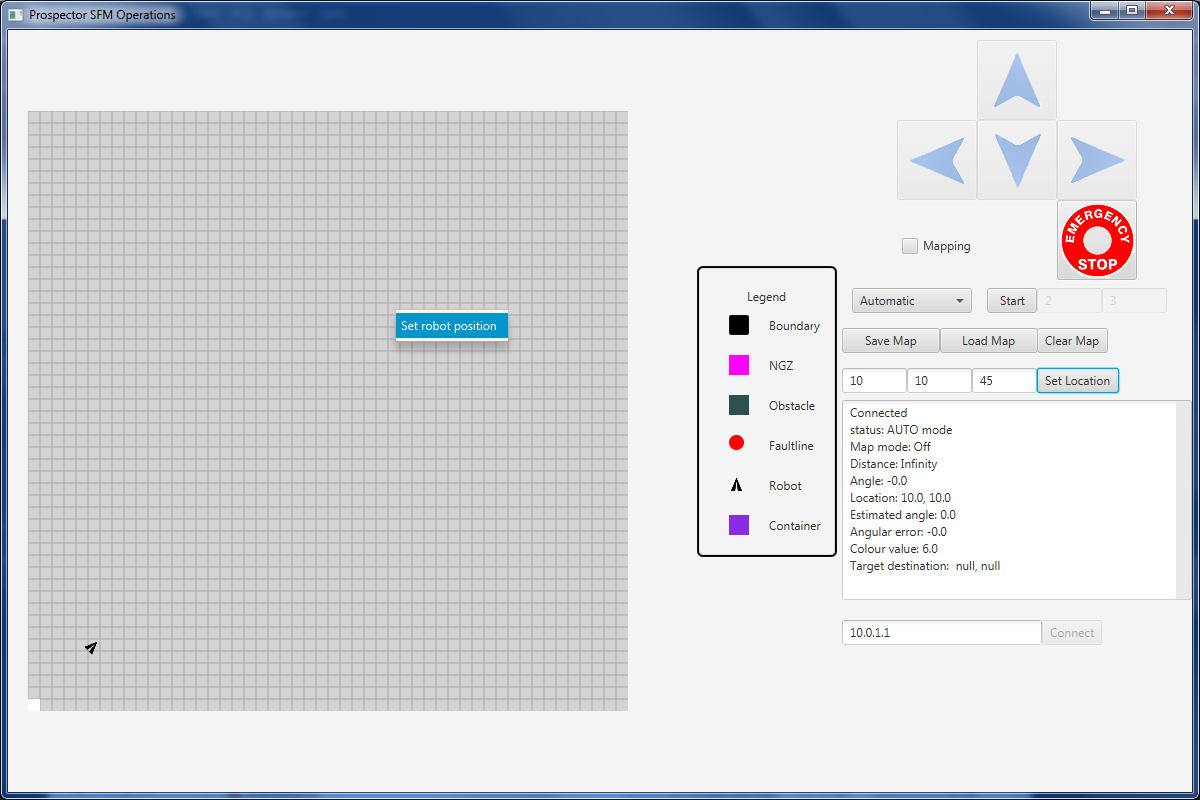
\includegraphics[width=15cm,height=15cm,keepaspectratio]{robot_position_rightclick_contextmenu.png}
\caption{Location Setting 1 }
  \label{fig:Location_setting1}
 \end{figure} 
  \begin{figure}[H] 
\centering
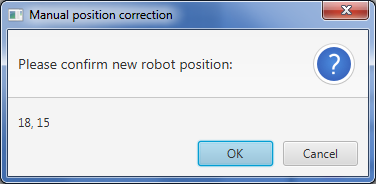
\includegraphics[width=10cm,height=10cm,keepaspectratio]{robot_position_rightclick_confirm.png}
\caption{Location Setting 2 }
  \label{fig:Location_setting2}
\end{figure}
\clearpage
\subsubsection{Information field}
The user interface provides the information about the robot, such as whether connect, the distance between the robot and obstacle, and the current location, show below:
\begin{figure}[H]
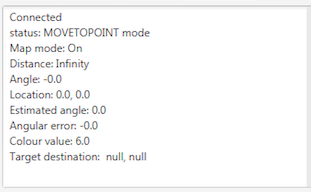
\includegraphics[width=\textwidth]{Information_field.png}
\caption{Information Field}
  \label{fig:Information_field}
\end{figure}


\subsubsection{Map legend}
The user interface provides the legend to demonstrate the label, for example, the black square means the bound, the pink square mean the no-go-zone, show below:
\begin{figure}[H]
\centering 
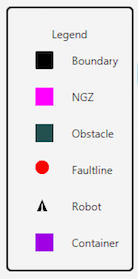
\includegraphics[width=10cm,height=10cm,keepaspectratio]{Legend.png}
\caption{Map Legend}
  \label{fig:Legend}
\end{figure}

\subsubsection{Map drawing}
The user interface provides an area to draw the map that robot detected in real-time, the map will be show as grid, users can check the robot's work, show below:
\ 
\begin{figure}[H]
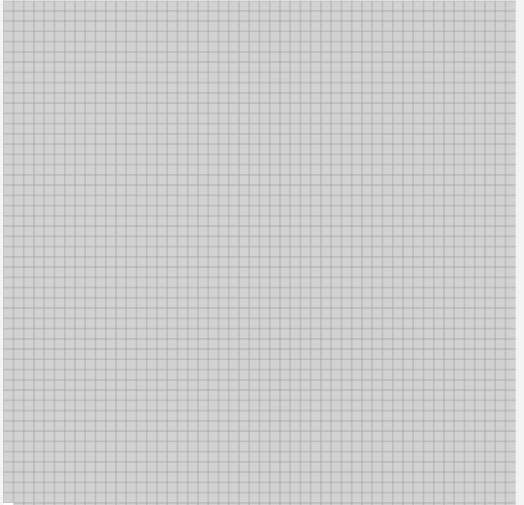
\includegraphics[width=\textwidth]{drawmap.png}
\caption{Map Grid}
  \label{fig:Map_grid}
\end{figure}

\subsubsection{Setting a No Go Zone }
The user interface allow user to mark a No Go Zone (NGZ) by choosing which area user want to make a NGZ. To Specify the NGZ area user just has to Select the area with left click on the Map grid and leave it will be marked as NGZ.
\begin{figure}[H]


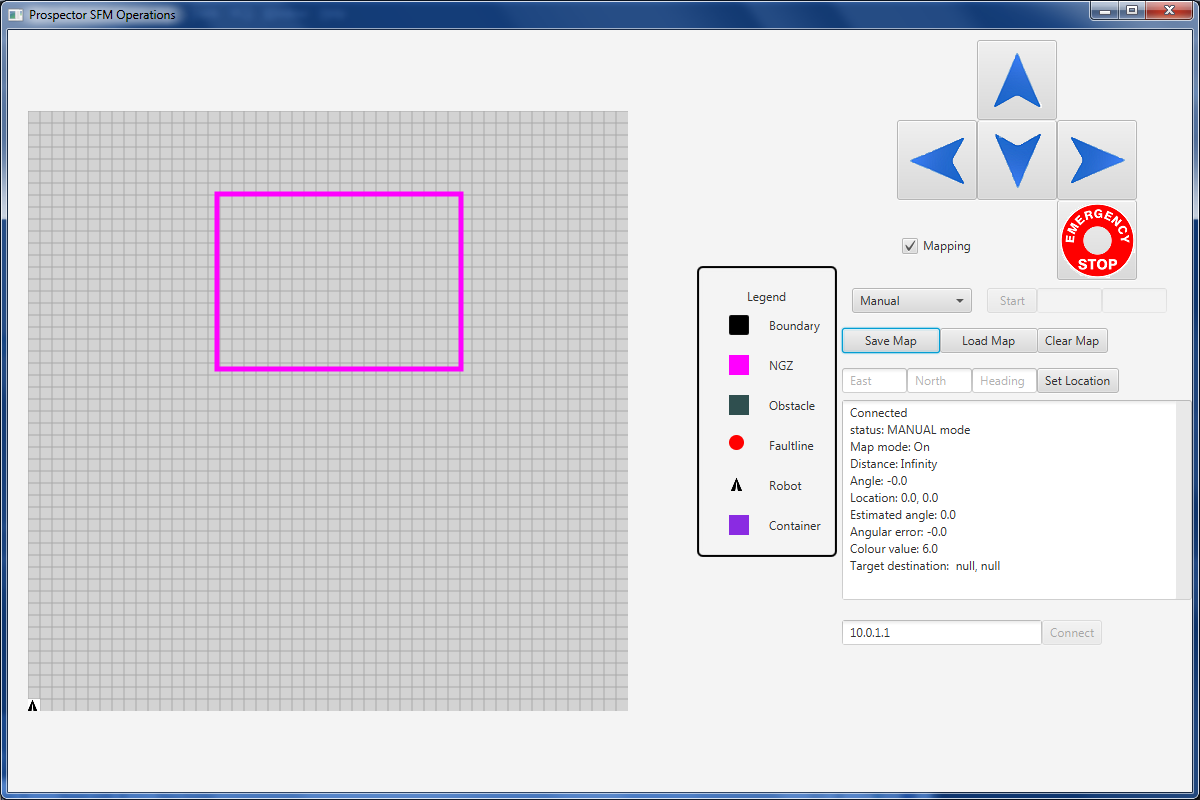
\includegraphics[width=\textwidth]{click_drag_ngz.png}
\caption{No Go Zone}
  \label{fig:No_go_zone}
\end{figure}




\begin{thebibliography}{1}


\bibitem{SRS} Prospector Team 2016. \textit{Software Requirements Specification: Prospector Seafloor Mapping System}. Version 0.1 (Draft).

\bibitem{SDD} Prospector Team 2016. \textit{Software Design Document: Prospector Seafloor Mapping System}. Version 1.0 (Draft).   

  \end{thebibliography}
\end{document}


